\documentclass{article}
\usepackage{arxiv}
\usepackage{graphicx}
\usepackage{amsmath}
\usepackage[round,authoryear]{natbib}
\usepackage{hyperref}

\title{Community Sorting Across Platforms}
\author{Colin Henry \\
  Department of Political Science, University of Zurich, Switzerland}
\date{}

\begin{document}

\maketitle

\begin{abstract}
Extremist communities do not simply get deplatformed and disappear; they cycle across the platform ecosystem---concentrating, raiding mainstream spaces, retreating, and re-entering. What structural features enable this pattern? I adapt the Tiebout model of citizen sorting to conceptualize platforms as quasi-governments offering public goods and communities as mobile citizen-voters choosing among governance regimes. Using an agent-based model with three simulation experiments in a $3 \times 3 \times 3$ factorial design crossing platform count, extremist proportion, and parasitism intensity, I find that the sorting mechanism is remarkably resilient to parasitism on average but breaks down under identifiable structural conditions. Three results emerge. First, platform diversification protects mainstream communities, and the premium grows with threat severity as the mechanism shifts from preference matching to target dilution. Second, coalition-based governance provides the strongest structural firewall: mediocre without extremists, it generates endogenous enclaves that sever the parasitism channel under threat. Third, the concentration--raid--retreat cycle is an emergent property of decentralized sorting, not coordinated strategy. The policy implication is that platform-system architecture---the mix of governance types and jurisdictional diversity---rather than individual moderation decisions, determines whether mainstream communities are structurally protected or exposed.

\textbf{Keywords:} social media platforms, community sorting, Tiebout model, content moderation, online extremism, agent-based modeling
\end{abstract}

\section{Introduction}

Extremist communities do not simply get ``deplatformed'' and disappear. Instead, many extremist movements appear to cycle across the platform ecosystem: they concentrate on sympathetic peripheral sites, coordinate harassment or recruitment efforts aimed at mainstream audiences, retreat when sanctioned, and then re-enter mainstream spaces when governance conditions change. This pattern is documented by researchers and journalists tracking organized off-site action, including coordinated returns to major platforms for messaging, recruitment, or harassment \citep{lavin2020culture, gais2021encrypted}. The empirical puzzle is not whether online communities move, but why extremist communities move \emph{in this particular way}---and what about the structure of the platform system enables or constrains these strategies \citep{dehghan2022politicization}.

I find three things. First, platform diversification protects mainstream communities, and the premium grows with extremist threat severity. Second, coalition-based governance provides structural immunity through endogenous enclave formation---paradoxically, the governance type that underperforms in benign conditions becomes the strongest firewall under threat. Third, the concentration--raid--retreat cycle is an emergent structural property: no extremist community plans it, but the architecture of the platform ecosystem is sufficient to produce it without coordination.

Existing research speaks to pieces of this puzzle, but it does not explain the \emph{system-level} movement patterns that make extremist cycling possible. The deplatforming literature largely treats platform access as a binary condition: actors are either on a mainstream platform or removed from it, after which attention shifts to evasion, reconstitution, or migration to alternative venues \citep{dehghan2022politicization}. Content-moderation and platform-governance research, by contrast, typically focuses on within-platform rulemaking and enforcement, emphasizing the discretionary and contested nature of moderation on general-purpose platforms \citep{klonick2017new}. Neither framework models how the \emph{mix} of platform types, governance structures, and community compositions creates incentives for extremist groups to concentrate, raid, retreat, and re-enter across multiple venues \citep{lavin2020culture, gais2021encrypted}.

More broadly, political communication work makes clear that where audiences are located matters for politics---platforms can facilitate mobilization and protest, shift public attention, enable surveillance and repression, and amplify or silence marginalized voices \citep{tufekci2017twitter, barberaDistractDivertHow2022, gohdesRepressionTechnologyInternet2020, panHowGovernmentcontrolledMedia2022, reny2021opinion, larson2019social, bonilla2020identity, pan2020saudi}. But these literatures rarely treat the platform ecosystem itself as an object of theory: a competitive environment in which communities endogenously sort across platforms, and in which changes in consolidation versus diversity, permissive versus exclusionary moderation, and governance mechanisms reshape the strategic interaction between extremists and mainstream communities. Explaining extremist cycling therefore requires a model of \emph{inter-platform dynamics}, not only intra-platform policy.

To model community sorting across a system of heterogeneous platforms, I adapt the Tiebout model of citizen sorting across jurisdictions \citep{tiebout1956pure}. Tiebout (1956) showed that if citizens can move freely among municipalities offering different bundles of public goods, they can ``vote with their feet,'' producing efficient sorting onto preferred jurisdictions. I reconceptualize platforms as quasi-governments offering public goods in the form of attention distribution to user-generated content (UGC), and communities as mobile citizen-voters choosing among these jurisdictions. This theoretical move captures two features missing from existing accounts: communities respond to a \emph{bundle} of governance choices rather than any single policy, and their movement decisions are shaped by the composition of the \emph{entire} platform system, not only the platform they currently occupy.

I adapt the Tiebout sorting model to this setting and conduct three simulation experiments. The first establishes baseline sorting dynamics; the second introduces extremist communities; the third traces the emergent raiding cycles that connect the cross-sectional and dynamic patterns.

The paper is organized as follows. Section~\ref{sec:puzzle} describes the empirical phenomenon the model is designed to explain. Section~\ref{sec:framework} develops the theoretical framework. Section~\ref{sec:results} presents the findings. Appendices~\ref{app:model} and \ref{app:design} contain the formal model specification and experimental design.

\section{The Sorting Puzzle}
\label{sec:puzzle}

Before developing the formal framework, it is worth dwelling on what the simulation actually reveals---three patterns striking enough to demand explanation.

\textbf{Extremists concentrate on direct platforms, stably and substantially.} Approximately 50\% of all extremist communities reside on direct-voting platforms at the end of each simulation, regardless of system size or threat intensity: 49\% at 5\% extremist prevalence, 50\% at 10\%, and 50\% at 15\%. Direct-voting platforms hold only 5--23\% of all communities depending on system configuration, so this represents a 3--10$\times$ overrepresentation relative to population share. This concentration holds across all levels of parasitism intensity and platform count. It does not drift or dissipate as the simulation runs; it is a stable attractor. The biography panels in Figure~\ref{fig:biography} illustrate the divergence: direct-platform community counts separate sharply from algorithmic and coalition platforms as parasitism intensity rises, while coalition platforms remain substantially buffered throughout.

\textbf{Movement is bursty, not continuous.} Extremist communities do not gradually drift across the platform ecosystem---they move in concentrated bursts. On direct platforms, 94--100\% of extremist outflow occurs in burst events (defined as ten or more departures in a single simulation step). The median burst involves 31 extremist communities. Median inter-burst intervals are approximately nine steps. The burst size distributions (Figure~\ref{fig:burst}) reveal that this pattern is robust across the $N_p \times \alpha$ factorial: bursts are large and frequent at high platform count and low parasitism, and remain frequent but shift in character as griefer behavior intensifies.

\textbf{Governance type produces a qualitative difference in welfare outcomes.} Mainstream welfare on coalition platforms declines by only 0.22 utility units as parasitism intensity rises from low ($\alpha = 2$) to high ($\alpha = 10$); on direct platforms, the decline is 3.60 units. This is not a difference of degree. Coalition platforms---which appear mediocre in benign conditions---provide structural immunity under threat. Direct platforms---which appear to be high-performing boutique spaces at low parasitism---become structurally exposed as the extremist threat intensifies. The governance type, not the threat level, determines which side of this divide a platform sits on.

How does this pattern emerge? No individual extremist community in the model plans the raiding cycle. The model contains no coordination mechanism---communities observe platform governance bundles but not social composition when choosing where to move. The concentration--raid--retreat pattern arises entirely from decentralized utility-maximizing behavior given the payoff structure of the platform ecosystem. The framework developed in Section~\ref{sec:framework} explains why.

\section{Framework}
\label{sec:framework}

The framework adapts the Tiebout model to the platform context. The full formal specification is in Appendix~\ref{app:model}; this section conveys the essential logic in plain terms and introduces the four equations that drive the results.

\subsection{Platforms as Quasi-Governments}

Tiebout's insight was that citizens can ``vote with their feet'': if they can move freely among municipalities offering different bundles of public goods, they sort themselves onto jurisdictions matching their preferences \citep{tiebout1956pure}. I apply this logic to online platforms. Platforms offer governance bundles---combinations of moderation rules, discourse architecture, and community autonomy features---and communities move when they can do better elsewhere.

Three types of governance regime are modeled. \textit{Direct voting} platforms aggregate community preferences through majority rule on each policy dimension. \textit{Coalition formation} platforms allow communities to form movements that propose alternative governance bundles, with the plurality winner replacing the current policy. \textit{Algorithmic recommendation} platforms use SVD-based grouping to deliver tailored bundles to clusters of communities with similar preferences. Each regime creates a different relationship between community composition and governance outcomes, and a different structure of exposure between extremist and mainstream communities.\footnote{Full formal specification of each mechanism is in Appendix~\ref{app:model}.}

\subsection{Two Kinds of Extremist Community}

Mainstream communities want platforms whose governance bundles align with their preferences. When no extremist communities are present, their utility is simply a function of how well the platform bundle matches their preference vector. When extremist communities arrive, mainstream communities suffer a utility penalty proportional to their exposure. The mainstream utility function is:

\begin{equation}
u_{c_m} = u_{\text{base}}(c_m, p) - \alpha \cdot \frac{N_{c_e}(c_m)}{N_{c_e}(c_m) + N_{c_m}(c_m)}
\label{eq:mainstream}
\end{equation}

\noindent where $u_{\text{base}}$ counts preference-bundle matches, $N_{c_e}(c_m)$ is the count of extremist neighbors, and $N_{c_m}(c_m)$ is the count of mainstream neighbors. The fraction is the extremist share of a community's neighborhood; $\alpha$ scales the maximum penalty.

Extremist communities extract utility from mainstream neighbors---they are ``utility vampires.'' Their utility function has the same structure but with the sign reversed on the social term:

\begin{equation}
u_{c_e} = u_{\text{base}}(c_e, p) + \alpha \cdot \frac{N_{c_m}(c_e)}{N_{c_m}(c_e) + N_{c_e}(c_e)}
\label{eq:griefer}
\end{equation}

\noindent The more mainstream neighbors an extremist community has, the higher its social payoff. The parameter $\alpha$ parameterizes the ideologue--griefer spectrum and is varied across $\{2, 5, 10\}$. At low $\alpha$, the social term contributes little to total utility, so extremists behave as \textit{ideologues}: they primarily seek platforms whose governance bundles align with their (maximally polarized) preferences. At high $\alpha$, the social term dominates, and the same communities become \textit{griefers}: they prioritize access to mainstream targets over policy alignment.

\subsection{Governance and Structural Exposure}

The definition of ``neighbor'' varies by governance type, and this variation is the key mechanism.

On \textit{direct platforms}, all communities on the platform are mutual neighbors under a single majority-rule bundle. There is no structural insulation: every extremist community has access to every mainstream community. On \textit{coalition platforms}, winning coalitions define neighborhoods---communities within the same coalition are neighbors, communities in different coalitions are not. This creates the potential for type-based segregation: if extremist and mainstream communities sort into separate coalitions, the parasitism channel is structurally severed. On \textit{algorithmic platforms}, SVD groupings define neighborhoods. Communities within the same algorithmically assigned group are neighbors; communities in different groups are not. This provides partial insulation, but new arrivals face the ``cold start'' problem: without sufficient interaction history, the algorithm may assign them to groups with dissimilar communities.\footnote{Full mechanism specifications are in Appendix~\ref{app:model}, \S A.3--A.4.}

Governance type therefore determines whether extremists have structural access to mainstream neighbors. The cross-sectional pattern documented in Section~\ref{sec:puzzle}---50\% concentration on direct platforms---follows directly from this structural logic.

\subsection{The Sorting Process}

Each simulation step proceeds as follows: governance updates the bundle, communities compute utility, communities search for better alternatives, and all relocations occur simultaneously. The key information restriction is that communities observe governance outputs (bundles) but not social composition when evaluating alternatives. An extremist community cannot identify target-rich platforms before arriving; a mainstream community cannot identify safe platforms before arriving. Any emergent patterns are the product of utility-maximizing behavior under incomplete information, not strategic foresight.

The search rule is:

\begin{equation}
p^* = \arg\max_{q \neq p} \; u_{\text{base}}(c, q)
\label{eq:search}
\end{equation}

\noindent Communities evaluate alternatives using only base utility---the match between their preferences and the candidate platform's bundle---because social composition is unobservable. A community moves if and only if base utility at the best alternative exceeds current full utility (including the social term). The simulation terminates at equilibrium or $t_{\max}$.

The formal model, governance algorithms, and experimental design are specified in Appendices~\ref{app:model} and \ref{app:design}.

\section{Results}
\label{sec:results}

The results are organized in five parts. Section~\ref{sec:results_exp1} establishes baseline sorting dynamics. Section~\ref{sec:results_diversification} shows that diversification protects and that protection grows with threat. Section~\ref{sec:results_governance} clusters the governance-type findings. Section~\ref{sec:results_raiding} reveals the dynamic mechanism. Section~\ref{sec:results_mixed} confirms the pattern under mixed extremist populations.

\subsection{Baseline Sorting: The Mechanism Translates}
\label{sec:results_exp1}

\subsubsection{Result 1: Governance type shapes sorting efficiency, but the ranking depends on system composition}

In homogeneous systems---where all $N_p = 9$ platforms share a single governance type---algorithmic platforms produce the highest average community utility (6.49), followed by coalition (6.06) and direct voting (5.40). The gap between algorithmic and direct exceeds 1.0 utility units, more than 10\% of the theoretical maximum. The mechanism is straightforward: algorithmic governance serves heterogeneous preferences simultaneously by constructing per-group content bundles, whereas direct voting forces a single majority-rule bundle on all tenant communities, imposing the full cost of preference misalignment on minority groups.

This ranking partially inverts, however, in mixed systems containing equal shares of all three governance types. When communities can sort freely across governance regimes, direct-voting platforms deliver the \textit{highest} per-capita utility: 6.31 at $N_p = 3$, 7.05 at $N_p = 9$, and 7.61 at $N_p = 27$. The explanation is selection. Most communities (59--76\%, increasing with $N_p$) migrate to algorithmic platforms, which offer acceptable utility to a wide range of preferences. The residual population on direct platforms is self-selected for preference alignment: communities that remain under majority rule do so because they share the majority preference. At $N_p = 27$, direct platforms hold only 4.8\% of all communities but deliver utility more than 1.0 units above the system average. Coalition platforms occupy a stable middle ground, attracting 19--20\% of communities across all system sizes, serving communities too heterogeneous for direct voting but preferring explicit coalition structure over opaque algorithmic recommendations.

This result establishes two baselines that Experiment~2 will complicate. First, algorithmic governance dominates in uniform systems but becomes a refuge platform in diverse ones. Second, direct-voting platforms function as high-utility boutique spaces---\textit{provided} their electorates are homogeneous. The question is what happens when that homogeneity is disrupted.

\subsubsection{Result 2: Platform diversification improves welfare}

System-wide utility increases monotonically with the number of available platforms: 6.20 ($N_p = 3$), 6.42 ($N_p = 9$), and 6.63 ($N_p = 27$). The gain is approximately 0.2 utility units per tripling of platforms, consistent across governance types. Variance simultaneously decreases (SD from 0.144 to 0.116), so diversification produces both higher and more equal outcomes. This is the core Tiebout prediction confirmed in the platform context: more jurisdictions allow finer-grained matching between community preferences and governance bundles.

The diversification premium is modest in absolute terms---roughly 7\% of system-average utility across the full range of $N_p$. This sets up the central question for Experiment~2: does the premium persist, shrink, or grow when some communities are parasitic?

\subsection{Diversification Protects---And More So Under Threat}
\label{sec:results_diversification}

\subsubsection{Result 3: The diversification premium grows with extremist threat}

The diversification premium---the welfare gain from more platforms---nearly doubles as parasitism intensity increases. Table~\ref{tab:divpremium} reports normalized mainstream utility at $\rho_e = 0.15$ across the $N_p \times \alpha$ grid.

\begin{table}[t]
\centering
\small
\begin{tabular}{lcccr}
\hline
 & $N_p = 3$ & $N_p = 9$ & $N_p = 27$ & $\Delta$(27 vs.\ 3) \\
\hline
$\alpha = 2$  & 0.593 & 0.619 & 0.642 & +0.049 \\
$\alpha = 5$  & 0.562 & 0.600 & 0.630 & +0.068 \\
$\alpha = 10$ & 0.511 & 0.567 & 0.609 & +0.098 \\
\hline
\end{tabular}
\caption{Normalized mainstream utility by platform count and parasitism intensity ($\rho_e = 0.15$). The diversification premium (rightmost column) nearly doubles from low to high parasitism.}
\label{tab:divpremium}
\end{table}

The small range of mean effects across the full factorial is itself evidence of resilience: the Tiebout mechanism absorbs parasitism without catastrophic welfare loss. The full range of mean normalized mainstream utility spans only 0.135 (from 0.511 at the worst-case configuration to 0.646 at the best). But the \textit{distribution} of those effects across system configurations tells a different story. The premium at $\alpha = 10$ reaches +0.098 [bootstrap 95\% CI: 0.093, 1.03 in raw utility units]. A difference-in-differences test comparing the premium at $\alpha = 10$ versus $\alpha = 5$ yields 0.29 [0.24, 0.35], confirming that the interaction is not merely additive.

A three-way ANOVA on normalized mainstream utility at $\rho_e = 0.15$ confirms that platform count and parasitism intensity are the dominant drivers: $N_p$ accounts for 47\% of variance ($\eta^2 = 0.47$, $F = 2{,}406$, $p < 0.001$) and $\alpha$ for 35\% ($\eta^2 = 0.35$, $F = 1{,}466$, $p < 0.001$). Their interaction contributes a further 6.4\% ($\eta^2 = 0.064$, $F = 92$, $p < 0.001$).\footnote{All ANOVA results are substantively identical at $\rho_e = 0.05$ and $\rho_e = 0.10$, with slightly smaller effect sizes for $\alpha$.}

The mechanism has shifted from Experiment~1. Without extremists, diversification improved welfare through finer preference matching. With extremists, an additional channel opens: \textit{target dilution}. More platforms spread extremist communities across a larger number of jurisdictions, reducing the parasitism density on any given platform. The welfare cost of platform consolidation thus depends on what kinds of communities inhabit the system, and the benefit of diversification is greatest precisely when the extremist threat is most severe.

\subsection{Governance Type Determines Structural Vulnerability}
\label{sec:results_governance}

The three results in this section form an analytical cluster. Result~6 establishes the most striking descriptive: extremists concentrate on direct platforms at 3--10$\times$ their population share. Result~4 explains why, through the behavioral regime shift that $\alpha$ produces. Result~5 identifies the protection mechanism on coalition platforms.

\subsubsection{Result 6: Extremists concentrate on direct platforms through endogenous selection}

Approximately 50\% of all extremist communities reside on direct-voting platforms at the end of each simulation, regardless of extremist proportion: 49\% at $\rho_e = 0.05$, 50\% at $\rho_e = 0.10$, and 50\% at $\rho_e = 0.15$. Since direct platforms hold only 5--23\% of all communities (depending on $N_p$ and $\alpha$), this represents a 3--10$\times$ overrepresentation relative to population share. The concentration is stable across all levels of $\alpha$ and $N_p$.

This concentration is not a parameter choice---it is an emergent selection equilibrium. Extremists are not assigned to direct platforms; they migrate there because direct voting offers the combination of capturable majority-rule governance and unprotected mainstream neighbors. On algorithmic platforms, the recommendation system partially insulates communities from neighbors with incompatible preferences. On coalition platforms, the enclave mechanism structurally separates extremists from targets (Result~5). Only direct-voting platforms leave all communities exposed under a single shared policy bundle, making them the optimal jurisdiction for parasitic extraction.

The stability of the 50\% concentration across all factor levels is striking. It suggests that the extremist sorting equilibrium is determined primarily by governance structure rather than by the intensity of parasitism or the total number of extremists in the system. Whether the system contains 45 or 135 extremist communities, half end up on direct platforms---the governance mechanism, not the threat level, sets the attractor.

\subsubsection{Result 4: Parasitism intensity produces qualitatively distinct behavioral regimes}

The parameter $\alpha$ does not simply scale extremist payoffs---it changes \textit{what extremists do}. At low parasitism intensity, extremists behave as ideologues: they seek platforms whose governance bundles align with their polarized preferences. At high intensity, the same communities become griefers, concentrating wherever mainstream targets are most accessible. This behavioral regime shift is visible in the divergent trajectories of direct-voting platforms across the $\alpha$ range.

At $\alpha = 2$ and $N_p = 27$, mainstream communities on direct platforms earn 5.84 average utility---below the system mean but well above the random baseline of 5.0. Direct platforms function as boutique spaces: high utility for well-matched residents, with extremists present but earning most of their payoff from policy alignment rather than parasitism. At $\alpha = 10$ and $N_p = 27$, however, mainstream utility on direct platforms collapses to 3.39---\textit{below} the random baseline. Extremist utility on the same platforms rises to 12.7--17.8, with the parasitism bonus dominating the base-match component of the utility function. Direct-voting platforms have shifted from boutique to vulnerable: the same governance mechanism that rewarded preference-aligned communities at low $\alpha$ now exposes unprotected mainstream communities to exploitation.

The regime shift is confirmed by tracking the ratio of extremist utility on direct versus algorithmic platforms. At $\alpha = 2$ ($N_p = 9$, $\rho_e = 0.10$), extremists earn 10.90 on direct platforms versus 6.91 on algorithmic, a ratio of 1.58. At $\alpha = 5$, the ratio rises to 1.65 (12.77 vs.\ 7.74); at $\alpha = 10$, to 1.67 (15.69 vs.\ 9.42). The growing premium that direct platforms offer to extremists reflects a shift in the composition of extremist payoffs: as $\alpha$ increases, the parasitism channel accounts for a larger share of total utility, and direct platforms---where all communities are neighbors under majority rule---become the optimal environment for extraction.

A counterintuitive detail underscores the structural nature of this failure mode. At $\alpha = 10$, mainstream utility on direct platforms is \textit{higher} in consolidated systems ($N_p = 3$: 4.62) than in diverse ones ($N_p = 27$: 3.39). The explanation is turbulence: with only three platforms, communities churn continuously, and no stable exploitation equilibrium forms. The high-$\alpha$, high-$N_p$ configuration is the worst case precisely because diversification allows extremists to settle into a stable concentration on direct platforms---the failure mode identified in Result~3's interaction term.

\begin{figure}[t]
  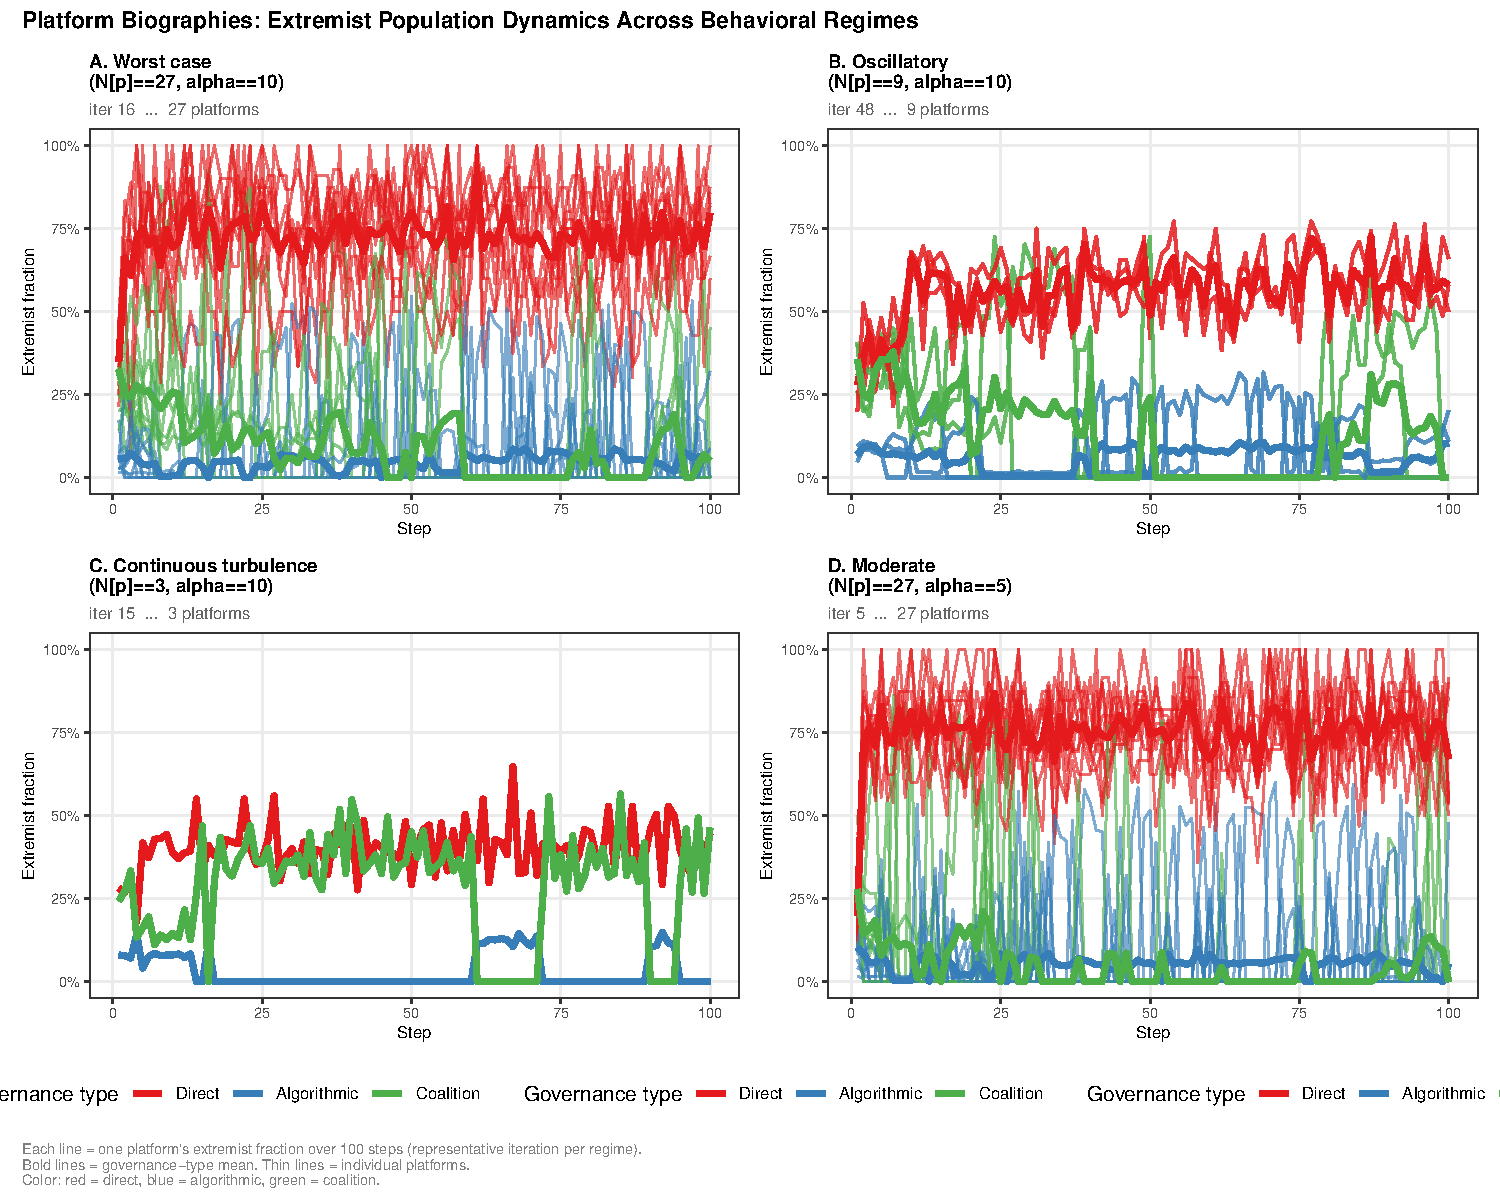
\includegraphics[width=\linewidth]{../../results/figures/biography_panel.pdf}
  \caption{Platform biography panels across four behavioral regimes. Bold lines show governance-type means; thin lines show individual platforms. Red: direct voting; blue: algorithmic; green: coalition. Top-left: worst case ($N_p = 27$, $\alpha = 10$); top-right: oscillatory ($N_p = 9$, $\alpha = 10$); bottom-left: continuous turbulence ($N_p = 3$, $\alpha = 10$); bottom-right: moderate ($N_p = 27$, $\alpha = 5$). Direct platforms diverge sharply from algorithmic and coalition as $\alpha$ increases.}
  \label{fig:biography}
\end{figure}

\subsubsection{Result 5: Coalition governance creates structural immunity through enclave formation}

Coalition-based governance provides the most stable mainstream welfare across the full range of parasitism intensity. Mainstream utility on coalition platforms declines by only 0.22 units as $\alpha$ increases from 2 to 10 (from 6.35 to 6.13), compared to a decline of 3.60 on direct platforms (from 7.01 to 3.41). This stability is not a product of excluding extremists from coalition platforms---extremists do arrive---but of the enclave mechanism that coalition governance produces.

On coalition platforms, communities form ideological blocs that jointly shift platform policy. Because coalitions aggregate preferences within groups, extremist and mainstream communities naturally sort into separate coalitions, each controlling different policy dimensions. Once this internal segregation occurs, the parasitism channel is structurally severed: extremists and mainstream communities are no longer effective neighbors. Mean coalition enclave homogeneity ranges from 0.92 to 0.98, with 74--92\% of simulation steps exceeding the 0.9 homogeneity threshold. The enclave mechanism is not instantaneous---settling takes a median of 23 steps at $N_p = 27$, $\alpha = 10$---but once established, it proves durable.

\begin{figure}[t]
  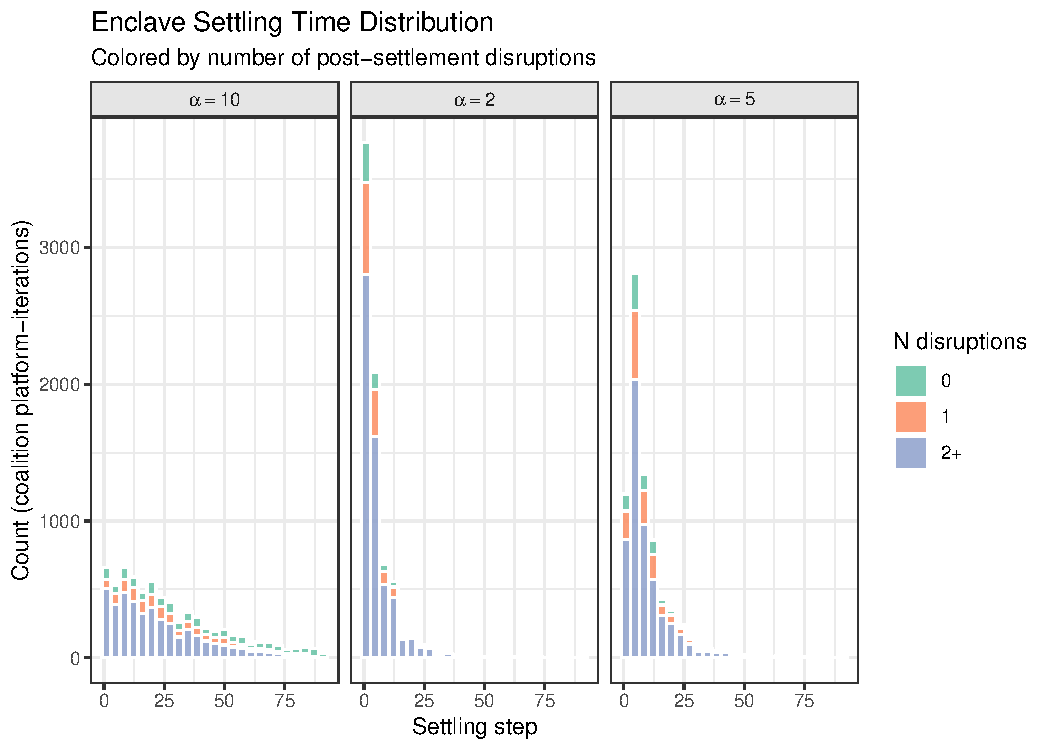
\includegraphics[width=\linewidth]{../../results/figures/enclave_settling.pdf}
  \caption{Histogram of coalition enclave settling steps, colored by the number of post-settlement disruptions (green: 0, orange: 1, blue: 2+), shown across three parasitism levels. At $\alpha = 2$ (center), enclaves form rapidly with a sharp modal peak near steps 1--3 and 2+ disruptions common even at low $\alpha$. At $\alpha = 5$ (right), the distribution broadens moderately. At $\alpha = 10$ (left), the settling distribution flattens substantially, extending beyond step 75, with 2+ disruptions prevalent throughout.}
  \label{fig:enclave}
\end{figure}

The temporal pattern reveals the mechanism's resilience. At low $\alpha$, enclaves form within the first five steps and experience at most one or two subsequent disruptions (Figure~\ref{fig:enclave}). At high $\alpha$, settling is delayed---the distribution of settling steps flattens, extending past step 90 in some iterations---and post-settlement disruptions become more frequent, typically coinciding with incoming raids from direct platforms. But the coalition mechanism re-sorts within a few steps of each disruption, restoring enclave homogeneity. The key insight is that coalition governance, which appeared mediocre without extremists (Result~1), turns out to be a natural firewall. The same movement-formation mechanism that made coalitions slower to converge in Experiment~1 now provides structural immunity against parasitic neighbors. Communities do not need to anticipate extremist behavior for the protection to emerge; the coalition structure produces it endogenously.

\subsection{Raiding Cycles Are Structural, Not Strategic}
\label{sec:results_raiding}

\subsubsection{Result 7: Extremist movement follows emergent raiding cycles}

On direct platforms, 94--100\% of extremist outflow occurs in burst events. The median burst involves 31 extremist communities. Median inter-burst intervals are approximately nine steps. These bursts are not strategic---they are the signature of a tipping dynamic operating on decentralized individual decisions.

The cross-sectional results above describe where extremists end up. The time-series evidence reveals \textit{how they get there}---through bursty, coordinated-looking movement events that are in fact emergent properties of the sorting process, not the product of strategic planning by any individual community.

The mechanism is a tipping dynamic: extremists accumulate on a direct platform, gradually shifting the policy bundle toward their polarized preferences. As the bundle shifts, mainstream communities suffer increasing parasitism costs and begin to depart. When enough mainstream communities leave, the parasitism payoff on that platform drops below the base-match utility available on algorithmic platforms, and a large group of extremists simultaneously discovers better options elsewhere---departing en masse, arriving on an algorithmic platform, temporarily disrupting its recommendation groupings, extracting utility from the mixed environment, and then dispersing as the algorithm re-sorts.

\begin{figure}[t]
  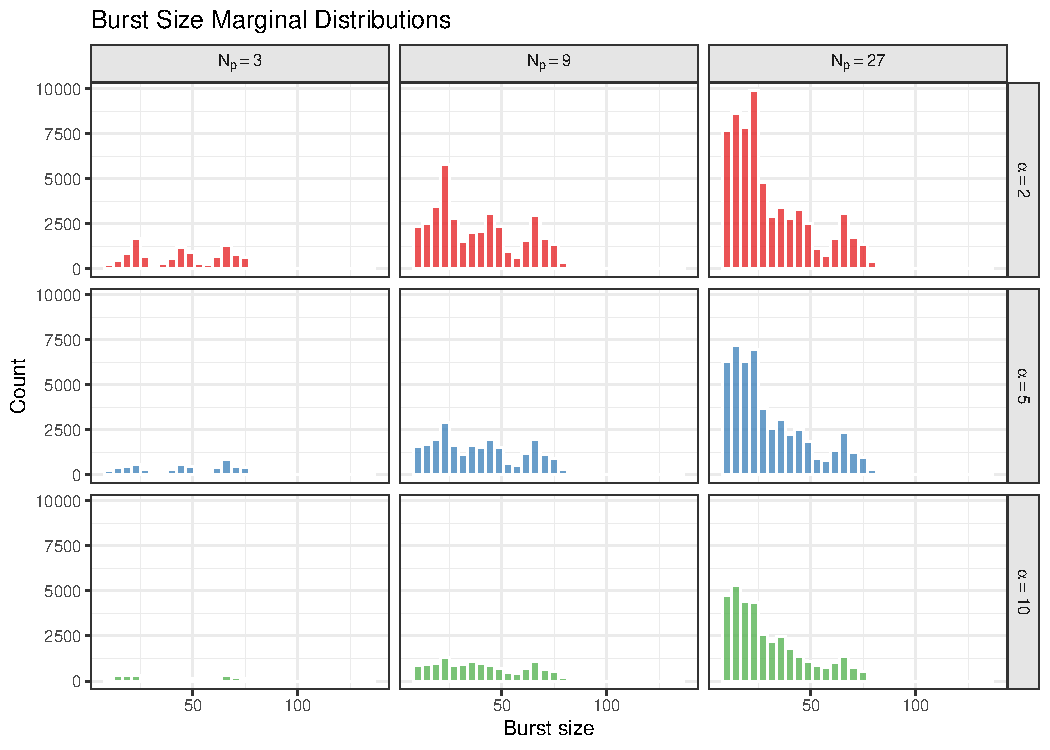
\includegraphics[width=\linewidth]{../../results/figures/burst_marginals.pdf}
  \caption{Burst size distributions across the $N_p \times \alpha$ factorial. Each panel shows the distribution of extremist burst sizes ($\geq 10$ departures per step). At $N_p = 3$ and $\alpha = 10$ (bottom-left), the panel is nearly empty: continuous turbulence replaces discrete bursts. At $N_p = 27$ and $\alpha = 2$ (top-right), bursts are large and frequent; at $N_p = 27$ and $\alpha = 10$ (bottom-right), bursts remain frequent but are concentrated at moderate sizes.}
  \label{fig:burst}
\end{figure}

\begin{figure}[t]
  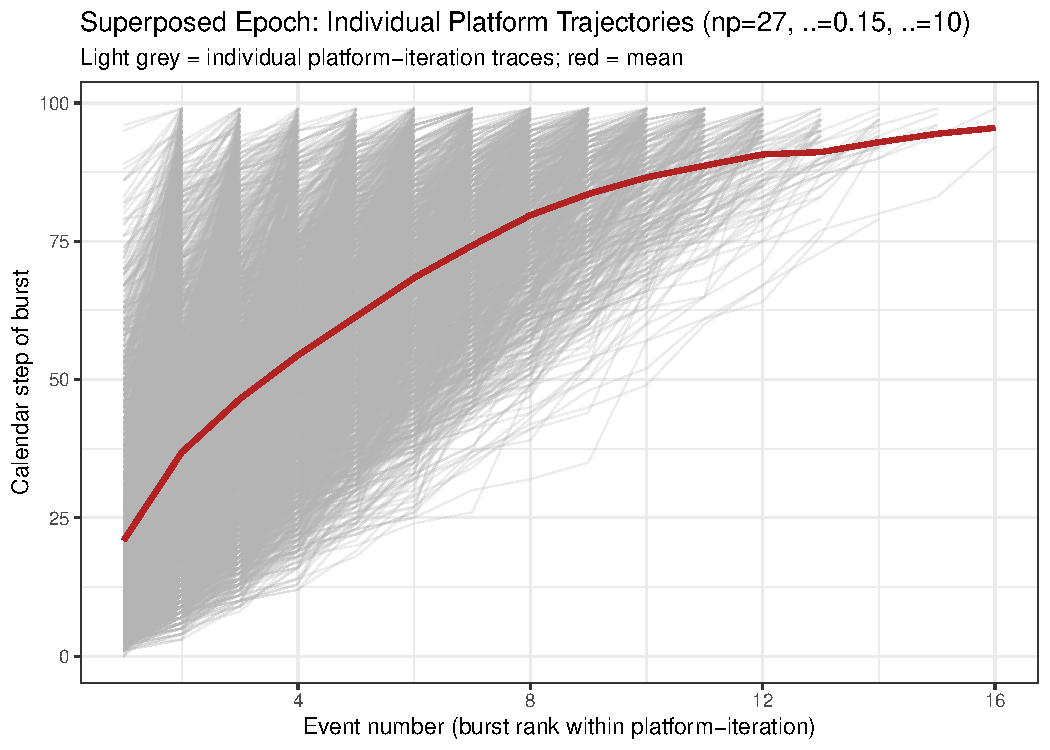
\includegraphics[width=\linewidth]{../../results/figures/spaghetti_epoch.pdf}
  \caption{Superposed epoch analysis of burst timing. Grey traces show individual platform trajectories; red line shows the mean across all platforms. Mean burst timing follows a log-deceleration pattern---each successive burst takes longer---but individual traces fan out widely, reflecting a bimodal population of platforms: those that stop experiencing bursts and those that continue.}
  \label{fig:spaghetti}
\end{figure}

The escalation dynamics of raiding differ sharply across system structures. At $N_p = 27$ and $\alpha = 10$, the mean per-platform escalation slope is 0.76 ($p = 0.008$)---statistically significant but modest, indicating gradual intensification. At $N_p = 3$ and $\alpha = 10$, the mean slope jumps to 15.1 ($p \approx 0$), reflecting continuous escalation in a turbulent system with few platforms. The superposed epoch analysis (Figure~\ref{fig:spaghetti}) reveals that the mean trajectory follows a log-deceleration pattern---each successive burst takes longer to arrive---but individual platform traces fan out widely. The distribution is bimodal: roughly 75\% of platforms show near-zero escalation slopes even at $\alpha = 10$, while the remaining 25\% exhibit strong positive escalation (Figure~\ref{fig:slope}). This heterogeneity is the signature of the failure mode: the system does not uniformly degrade, but a subset of direct platforms absorb disproportionate raiding pressure.

\begin{figure}[t]
  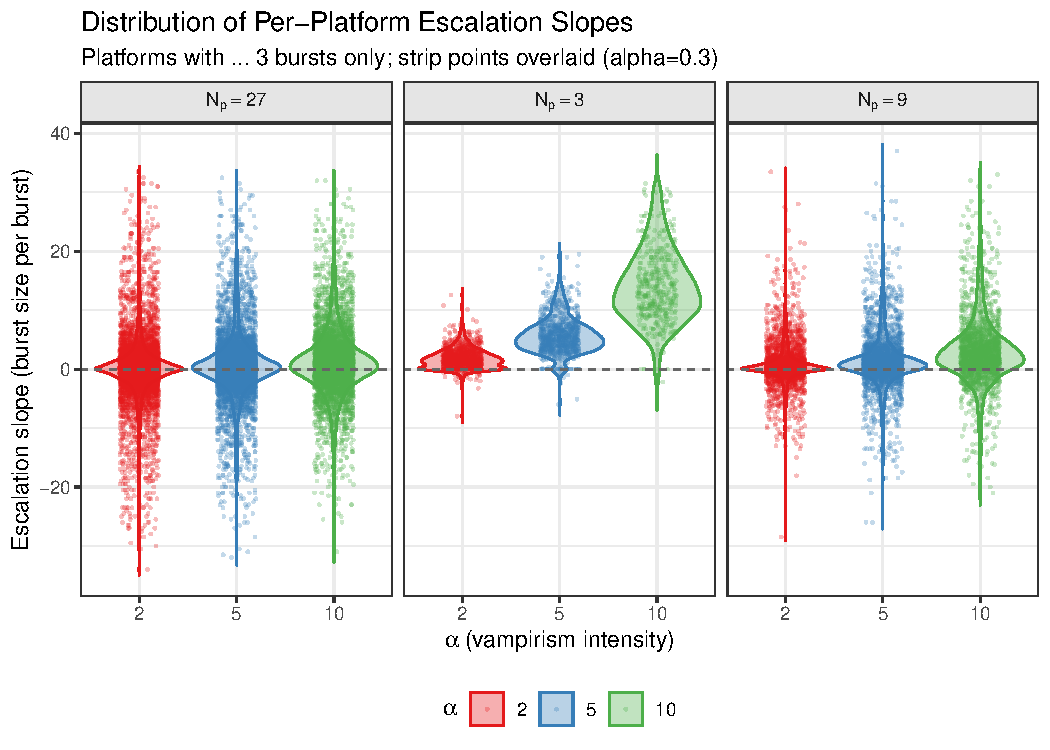
\includegraphics[width=\linewidth]{../../results/figures/slope_distribution.pdf}
  \caption{Distribution of per-platform escalation slopes across the $3 \times 3$ factorial. Each panel shows one level of $N_p$ (columns: $N_p \in \{3, 9, 27\}$); $\alpha$ varies along the x-axis within each panel. At low $\alpha$, slopes cluster tightly near zero across all $N_p$ conditions. At high $\alpha$, the distribution widens substantially---particularly at $N_p = 3$---with a subset of platforms showing strong positive escalation while the majority remain near zero, consistent with the bimodal pattern in which approximately 25\% of direct platforms absorb disproportionate raiding pressure.}
  \label{fig:slope}
\end{figure}

A final detail reinforces the resilience frame. The biography data reveal a displacement paradox: when raids displace mainstream communities from direct platforms, those communities typically land on platforms offering better preference matches. The mean displacement utility delta is +0.044 at $N_p = 27$, $\alpha = 10$, and no displacement events produce negative utility changes at this configuration ($\text{frac\_negative} = 0.00$). At $N_p = 3$, where turbulence limits sorting options, 6.1\% of displacements are negative---small but nonzero. Raids are costly for the direct platforms that experience them, but the system as a whole absorbs the shock: displaced communities find better homes, and short-term system utility marginally \textit{improves} after each burst. The Tiebout mechanism self-corrects, provided there are enough platforms to absorb the displaced.

\subsection{Mixed Populations Confirm the Pattern}
\label{sec:results_mixed}

\subsubsection{Result 4b: The behavioral regime generalizes to mixed extremist populations}

These results hold when the extremist population is a realistic mixture of ideologues and griefers rather than a pure type. Result~4 established the ideologue-griefer distinction under pure-type populations. Experiment~2b tests whether that distinction holds when the two subtypes are mixed within a fixed extremist share ($\rho_e = 0.10$, $N_p = 9$, $t_{\max} = 100$, 200 iterations per configuration). Griefer fraction $f_g \in \{0.25, 0.50, 0.75\}$ varies across three intermediate configurations, anchored at $f_g = 0$ (pure ideologues, $\alpha_i = 2$) and $f_g = 1$ (pure griefers, $\alpha_g = 10$) from the exp2 baselines. The three narrative results are reported in turn.

\paragraph{Welfare degradation is monotone in $f_g$ but governance-type-specific.}
Mainstream welfare declines continuously across the full $f_g$ gradient on all three governance types (Figure~\ref{fig:exp2b_governance}), but the magnitude of that decline differs sharply by institution. On direct platforms, welfare falls from 6.55 at $f_g = 0$ to 4.52 at $f_g = 1.00$, a loss of 2.03 utility units. On coalition platforms the corresponding loss is 0.34 (6.09 to 5.75); on algorithmic platforms, 0.31 (6.22 to 5.91). Direct platforms bear nearly the entire cost of the griefer gradient while coalition and algorithmic platforms remain substantially buffered throughout.

The damage on direct platforms is front-loaded. At $f_g = 0.25$---a population in which griefers constitute 25\% of an already-minority extremist group, or approximately 2.5\% of all communities---mainstream welfare on direct platforms has already fallen to 6.01, capturing the majority of the degradation ultimately observed at $f_g = 1.00$. Coalition welfare at the same point is 5.92 and algorithmic welfare 6.10, both close to their respective $f_g = 0$ baselines. This pattern sharpens the interaction finding from Result~3: the worst-performing configuration is produced disproportionately by the griefer subpopulation, and direct-voting governance is the institutional locus of that failure.

\begin{figure}[t]
  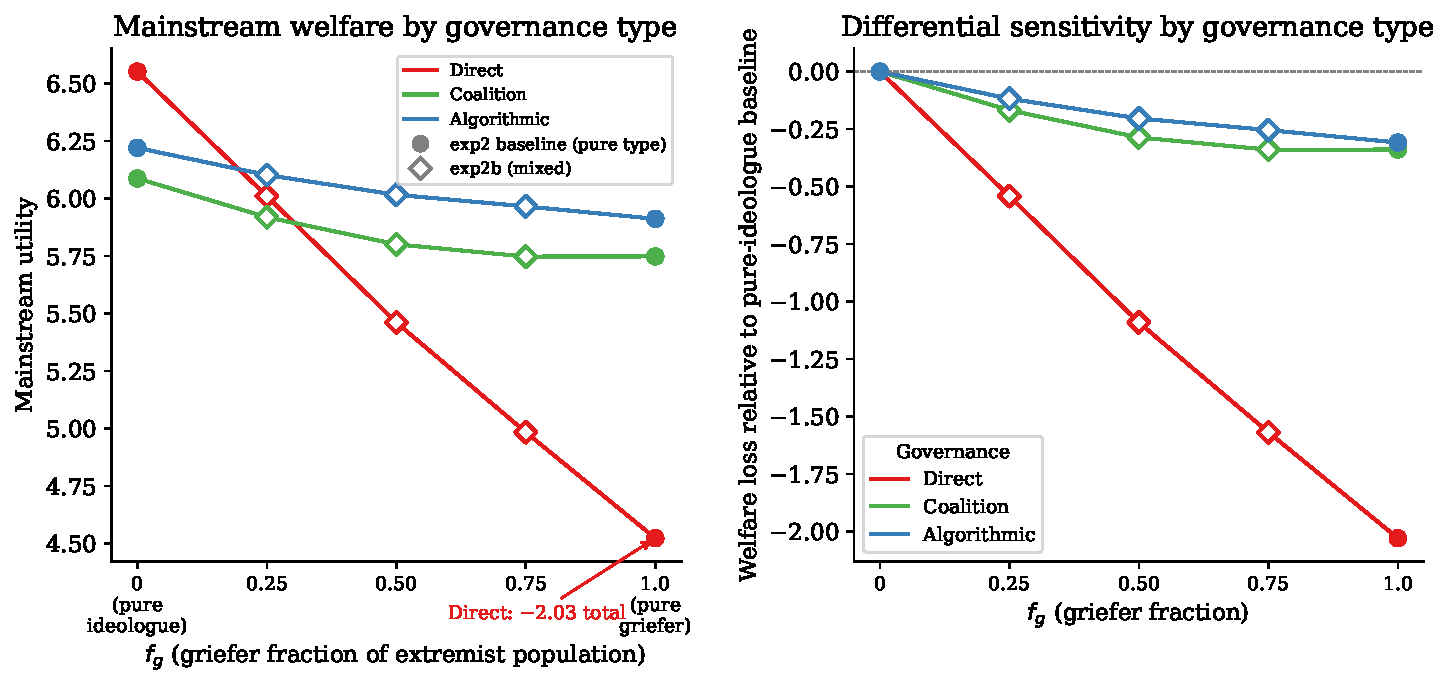
\includegraphics[width=\linewidth]{../../results/figures/exp2b_governance.pdf}
  \caption{Mainstream welfare by governance type across the griefer fraction gradient ($N_p = 9$, $\rho_e = 0.10$). Left: absolute mainstream utility (direct: red; coalition: green; algorithmic: blue). Right: welfare loss relative to the pure-ideologue baseline ($f_g = 0$). Filled circles indicate exp2 baseline endpoints; open diamonds indicate exp2b intermediate configurations. Direct-platform welfare declines 2.03 units across the $f_g$ range; coalition and algorithmic platforms lose 0.34 and 0.31 units respectively.}
  \label{fig:exp2b_governance}
\end{figure}

\paragraph{Burst dynamics shift from concentrated to escalating as $f_g$ increases.}
The change in burst structure across the $f_g$ gradient is qualitative, not merely a rescaling (Figure~\ref{fig:exp2b_dynamics}). At $f_g = 0.25$, raiding produces large, concentrated bursts (median 31 communities) with no significant time-trend in escalation (slope $= 0.07$, $p = 0.34$). As $f_g$ increases, burst size declines monotonically while escalation slope rises sharply: at $f_g = 0.50$, slope $= 0.24$ ($p = 0.001$); at $f_g = 0.75$, slope $= 1.27$ ($p < 0.001$). Ideologue-dominated populations produce policy-driven mass departures---large, discrete bursts when a platform's governance bundle no longer matches preferences. Griefer-dominated populations produce repeated low-grade disruption---smaller but escalating bursts as communities continuously seek accessible mainstream targets regardless of bundle. The $f_g$ gradient traces the continuous transition between these two regimes.

\paragraph{Enclave formation is slowed but not defeated by mixed extremist populations.}
Coalition enclave settling time rises from a mean of 21.8 steps at $f_g = 0.25$ to 39.7 steps at $f_g = 0.75$. At $f_g \geq 0.50$, at least 10\% of iterations do not achieve enclave equilibrium within $t_{\max} = 100$ (convergence mode: \textsc{still\_climbing}; 90th-percentile settling step $= 100$), a convergence failure absent at $f_g = 0.25$. Enclave homogeneity declines from 0.94 to 0.92 across the same range, remaining high throughout. The enclave mechanism is not defeated by mixed extremist populations; it is slowed. This qualification matters for Result~5's protection claim: coalition governance provides structural immunity, but the timeline for that immunity to materialize is longer when griefers constitute a larger share of the extremist population.

\begin{figure}[t]
  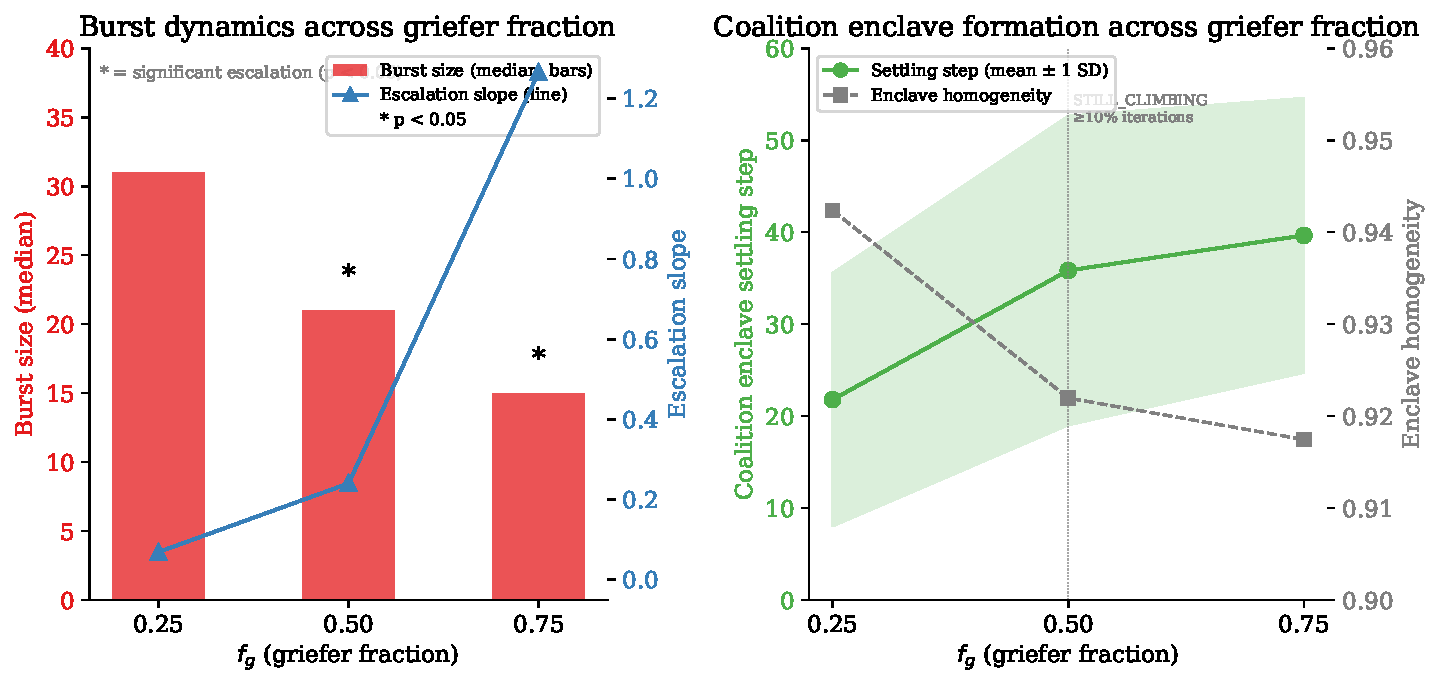
\includegraphics[width=\linewidth]{../../results/figures/exp2b_dynamics.pdf}
  \caption{Burst and enclave dynamics across the griefer fraction gradient ($N_p = 9$, $\rho_e = 0.10$). Left: median burst size (red bars, left axis) and escalation slope (blue line, right axis) at $f_g \in \{0.25, 0.50, 0.75\}$; asterisk indicates significant escalation ($p < 0.05$). Right: coalition enclave settling time (mean $\pm$ 1 SD, green line and ribbon, left axis) and enclave homogeneity (dashed grey, right axis). The vertical dashed line at $f_g = 0.50$ marks the onset of convergence failure in $\geq 10\%$ of iterations.}
  \label{fig:exp2b_dynamics}
\end{figure}

\paragraph{Validation of the $\alpha$ proxy.}
These results validate the use of $\alpha$ as a continuous behavioral proxy in the main factorial design. The ideologue-griefer transition is smooth and continuous in both welfare outcomes and burst dynamics across the $f_g$ gradient; the distinction between the two subtypes is not categorical. The intermediate value $\alpha = 5$ used in exp2 corresponds behaviorally to realistic mixed populations rather than a degenerate special case. The composite $\rho_e$ parameter, which conflates ideologue and griefer counts at fixed $\alpha$, is therefore a reasonable simplification for the factorial design. The $f_g$ results confirm that the simplification does not produce qualitatively misleading results.

\section{Discussion}
\label{sec:discussion}

The central finding of this paper is that the Tiebout sorting mechanism is remarkably resilient to parasitism. When extremist communities capable of extracting utility from mainstream neighbors enter a diverse platform ecosystem, the sorting process absorbs the threat without catastrophic welfare loss: the full range of normalized mainstream utility across the entire factorial spans only 0.135, a margin that would be difficult to distinguish from noise in most empirical settings. Communities displaced by extremist raids typically land on better-matched platforms, and the system self-corrects after each disruption. This resilience, however, is not unconditional. The model identifies a specific structural failure mode---the intersection of high parasitism intensity, direct-voting governance, and sufficient platform diversity for extremists to form stable exploitation equilibria---under which a subset of platforms absorbs disproportionate harm while the rest of the system appears healthy. The policy-relevant story is therefore not about average damage but about the conditions under which structural protection breaks down and the communities least equipped to defend themselves bear concentrated costs.

\subsection{Platform Design and the Consolidation Problem}

The diversification premium---the welfare gain from expanding the number of available platforms---is one of the most robust findings in the simulation. More platforms produce better outcomes, lower variance, and finer preference matching, consistent with the core Tiebout prediction. What the extremism experiments add is that this premium is not merely additive: it grows with the severity of the threat. The premium nearly doubles from low to high parasitism intensity, and the mechanism shifts from preference matching (which dominates in benign environments) to target dilution (which dominates under threat). More platforms spread extremist communities across more jurisdictions, reducing parasitism density on any given platform and preserving the sorting mechanism's ability to match mainstream communities with compatible governance.

This finding speaks directly to the contemporary platform landscape. The social media ecosystem is not characterized by the jurisdictional diversity that the Tiebout mechanism requires. A small number of firms---Meta, TikTok, Google---command the vast majority of user attention, and market dynamics continue to push toward consolidation rather than diversification. Scholars of media systems have long argued that viewpoint diversity depends on structural diversity in the media landscape \citep{tufekci2017twitter}; the model adds a sharper claim. Platform consolidation does not merely reduce preference matching---it systematically worsens outcomes for mainstream communities, and the magnitude of the harm scales with the extremist threat present. In a benign environment, consolidation leaves modest utility on the table. In a hostile one, it erodes the structural buffer that protects mainstream communities from parasitic exploitation. The tension is structural: the Tiebout mechanism requires a minimum of jurisdictional diversity to function, but the network effects and economies of scale that characterize platform markets push relentlessly toward consolidation.

Two qualifications temper this implication. First, the model's effects are modest on average. Consolidation alone does not produce catastrophe; it removes the system's capacity to absorb shocks when they arrive. The case for platform diversity is therefore less about preventing everyday harm and more about preserving structural resilience against tail-risk events---the platform equivalent of maintaining biodiversity not for its average-day benefits but for its insurance value. Second, the model treats platforms as passive and homogeneous within governance type. Real platforms differ in scale, network effects, content niche, and strategic behavior in ways that complicate a simple ``more is better'' prescription. The theoretical prediction is that jurisdictional diversity is protective; the policy translation requires attention to what kinds of new platforms would actually absorb communities and dilute extremist density, rather than simply fragmenting audiences across functionally identical services.

\subsection{Governance Design and the Coalition Paradox}

Coalition-based governance emerges as the strongest structural firewall against parasitic exploitation, and it does so through a mechanism that is genuinely counterintuitive. In the baseline experiments without extremists, coalition platforms appeared mediocre---slower to converge, lower in average utility than algorithmic platforms, and attracting a stable but unremarkable share of communities. Only when extremists entered the system did the coalition mechanism reveal its protective value. Mainstream utility on coalition platforms declined by just 0.22 units across the full range of parasitism intensity, compared to a decline of 3.60 on direct-voting platforms. The mechanism is enclave formation: coalition governance induces communities to form ideological blocs that jointly control policy dimensions, and this internal structure naturally segregates extremist and mainstream communities into separate coalitions. Once segregated, the parasitism channel is structurally severed---extremists and mainstream communities are no longer effective neighbors even when they share the same platform.

This enclave mechanism provides a structural analog to what the moderation literature describes as community self-governance. Platforms that support movement-formation tools---coalition voting, co-moderation, community-created rules---enable communities to construct internal boundaries that insulate members from hostile neighbors. The finding resonates with empirical observations from platforms like Reddit and Discord, where subreddit and server structures allow communities to establish and enforce their own norms, and where the most stable communities are those with the strongest internal governance \citep{chandrasekharan2017you}. The model suggests that the protective value of these structures derives not from their moderation rules per se but from the coalition-formation process itself: the act of aggregating preferences within blocs produces ideological coherence that extremists cannot easily penetrate.

The practical implication is that governance mechanisms supporting coalition formation---community voting systems, co-moderation structures, movement-building tools---may be more protective than either algorithmic sorting or direct majority rule. Algorithmic platforms serve as effective refuges in mixed systems, absorbing the largest share of communities and delivering acceptable utility to heterogeneous preferences. But they do not actively protect against parasitism; they merely dilute it. Direct-voting platforms, by contrast, shift from boutique to vulnerable as parasitism intensifies: the same governance mechanism that rewarded preference-aligned communities at low threat levels exposes unprotected mainstream communities to exploitation at high ones. Coalition governance occupies a distinct structural position---it actively generates protection through endogenous segregation, and this protection strengthens rather than weakens as the threat grows.

A significant limitation applies here. The model assumes that community coalitions can form organically---that communities possess the information, motivation, and institutional support to identify compatible partners and negotiate joint control of policy dimensions. Real platforms vary enormously in how much they support this process. Many mainstream platforms offer no coalition-formation mechanisms at all, relying entirely on algorithmic personalization or platform-level policy. The finding therefore identifies a design principle---governance that supports community-level coalition formation is structurally protective---rather than a description of existing platform behavior.

\subsection{Extremist Strategy as a System Property}

The empirical puzzle that motivated this paper---why extremist movements cycle across platforms in the specific pattern of concentration, raiding, retreat, and re-entry---receives a structural explanation from the simulation results. The raiding pattern is an emergent property of the sorting process under mixed governance, not the product of strategic planning by any individual community. No extremist community in the model plans a raid cycle; the cycle emerges from individual utility-maximizing moves given the payoff structure of the platform ecosystem. Extremists accumulate on direct-voting platforms where unprotected mainstream neighbors offer parasitic payoffs, gradually shift platform policy toward their preferences, drive mainstream communities out, experience declining parasitic returns, and then disperse to platforms where new targets are available. The cycle repeats because the structural conditions that produced it persist.

The simulation results further reveal that parasitism intensity does not merely scale the magnitude of extremist harm---it produces qualitatively distinct behavioral regimes. At low intensity, extremists behave as ideologues, seeking platforms whose governance bundles align with their polarized preferences. At high intensity, the same communities become griefers, concentrating wherever mainstream targets are most accessible regardless of policy alignment. This regime shift means that the character of the extremist threat, not just its magnitude, changes with the structural conditions of the ecosystem.

This finding reframes how we interpret empirically observed cross-platform coordination. Episodes like the Kiwi Farms harassment campaigns, GamerGate-era cross-platform mobilization, and recurring patterns of extremist return to mainstream spaces after deplatforming look planned, and some coordination certainly occurs. But the model suggests that much of this cycling behavior can arise from purely structural incentives: given a platform ecosystem containing direct-voting platforms with unprotected mainstream neighbors, the raiding pattern is a structural-incentive account sufficient to generate the pattern. The distinction matters for policy. If cycling is purely strategic, then disrupting coordination channels---encrypted messaging, off-platform planning spaces---should break the cycle. If cycling is substantially structural, then disrupting channels alone is insufficient; the cycle will re-emerge as long as the ecosystem contains the governance configurations that sustain it.

The displacement paradox reinforces this structural interpretation. When raids displace mainstream communities from direct platforms, those communities typically find better matches elsewhere---mean displacement utility is positive, and at high platform diversity no displacement events produce negative utility changes. The Tiebout mechanism self-corrects: raids are costly for the platforms that experience them but beneficial, in net, for the displaced communities and the system as a whole. This self-correction is itself a form of resilience, and it depends on the same jurisdictional diversity identified in the diversification results. At low platform counts, where sorting options are scarce, displacement occasionally produces negative outcomes. The system's capacity to absorb raiding shocks is a function of its structural diversity, closing the loop between the consolidation and extremist-strategy findings.

The policy implication is that deplatforming from a single venue does not break the extremist cycle if the ecosystem conditions---direct-voting platforms with unprotected mainstream neighbors, sufficient platform diversity for re-entry---persist elsewhere in the ecosystem. Effective intervention requires attention to the architecture of the platform system, not only to the moderation decisions of individual platforms.

\subsection{Limitations}

Several modeling choices constrain the scope of these findings. First, community preferences are fixed throughout each simulation. Real communities update their preferences in response to platform experiences, including exposure to extremist content, and preference dynamics could amplify or dampen the sorting patterns observed here. Second, platforms are passive actors: governance type is assigned and does not change. Real platforms strategically adjust their moderation, algorithms, and features to attract or repel communities, and these adjustments would introduce feedback loops absent from the current model. Third, the three governance types---direct voting, coalition formation, and algorithmic recommendation---are stylizations of a much more complex reality. Most real platforms combine elements of all three, and the boundaries between types shift over time as platforms redesign their systems.

Fourth, while the experimental design specifies planned sensitivity analyses, those results are not yet reported. The robustness of the core findings to alternative parameterizations, utility functional forms, and movement rules remains to be confirmed. Appendix~\ref{app:sensitivity} provides the planned sensitivity analysis specification; results from the OAT HPC run will be reported in a subsequent update. Fifth, the parameter ranges for platform count, extremist proportion, and parasitism intensity are theoretically motivated but not calibrated to specific real-world platforms or communities. The model is a theoretical device for identifying structural mechanisms, not a predictive tool for forecasting outcomes in particular platform ecosystems. These limitations are characteristic of the exploratory modeling tradition in which this work sits \citep{bankesExploratoryModelingPolicy1993}: the aim is to build theory and identify mechanisms that can guide empirical inquiry, not to generate point predictions.

\section{Conclusion}
\label{sec:conclusion}

This paper began with an empirical puzzle: why do extremist communities cycle across the platform ecosystem in the specific pattern of concentration, raiding, retreat, and re-entry? The deplatforming literature treats platform access as binary, and the moderation literature focuses on within-platform governance. Neither framework explains the system-level dynamics that make cycling both rational and emergent. The modified Tiebout model developed here provides a structural-incentive account sufficient to generate the pattern. Community sorting across a system of heterogeneous platforms produces an equilibrium in which extremists endogenously concentrate on direct-voting platforms, exploit unprotected mainstream neighbors, and disperse when parasitic returns decline---generating the cycling pattern as a structural property of the ecosystem rather than a product of coordinated strategy.

The theoretical contribution is to extend the Tiebout framework to multi-governance platform ecosystems and to identify the structural conditions under which parasitic exploitation becomes self-sustaining. The policy contribution is to redirect attention from individual moderation decisions to the architecture of the platform system itself. It is the mix of governance types, the degree of jurisdictional diversity, and the availability of coalition-formation mechanisms that determine whether mainstream communities are structurally protected or structurally exposed. Future work should pursue empirical calibration against observed platform migration data, introduce dynamic governance that allows platforms to respond strategically to community composition, and model preference updating to capture the feedback between extremist exposure and community radicalization.
\newpage

\bibliographystyle{plainnat}
\bibliography{refs}

% ============================================================
% APPENDICES
% ============================================================

\appendix

\section{Formal Model Specification}
\label{app:model}

I model community sorting across social media platforms as a modified Tiebout process. \cite{tiebout1956pure} argued that if citizens can move freely between municipalities offering different bundles of public goods, they sort themselves efficiently onto jurisdictions matching their preferences. Subsequent refinements have relaxed or extended the original assumptions in various ways \citep{bewley1981critique, wooders1994large, konishi1996voting}. Following this work, I adapt the Tiebout framework to a system of online platforms, reconceptualizing platforms as quasi-governments offering public goods in the form of attention distribution to user-generated content, and communities as mobile agents choosing among these jurisdictions. Two features of the online setting make the Tiebout framework especially apt: movement between platforms is low-cost relative to physical relocation between municipalities, and the ``public goods'' offered by platforms---content moderation rules, discourse architecture, community autonomy---are experienced collectively by all tenant communities.

The model proceeds in three stages. First, I define the agents (communities and platforms), the structure of the public good space, and the utility functions that govern community behavior (\S\ref{sec:agents}--\ref{sec:utility}). Second, I specify three platform governance mechanisms that determine how public good bundles change in response to community composition (\S\ref{sec:governance}). Third, I describe the Tiebout cycle: the sequence of governance updates, utility calculations, search, and relocation that constitutes a single simulation step (\S\ref{sec:cycle}). I close with a brief discussion of how each model component maps to observable features of real platforms (\S\ref{sec:mapping}).

\subsection{Agents and Environment}
\label{sec:agents}

\textbf{Communities.} Let $\mathcal{C} = \{c_1, \ldots, c_{N_c}\}$ be a set of $N_c$ communities. Each community is a unitary agent with a preference vector $B_c \in \{0,1\}^{N_a}$, where $N_a$ is the dimensionality of the public good space. Each binary element $b_{ca}$ represents a preference over a specific platform governance decision: whether to amplify or suppress a type of content, enable or disable a community management feature, and so forth. Communities are given and exogenous to the model; I do not model community formation, dissolution, or internal preference change.\footnote{Online communities are, of course, not unitary actors. Membership is fluid, identities are multiple, and intra-community preference aggregation is itself a complex process \citep{stryker2004integrating, stets2000identity}. I adopt the unitary actor assumption because the model's focus is platform-community interaction, not intra-community dynamics. This trades precision at the community level for tractability at the system level, a trade-off familiar from structural models in international relations \citep{waltzEvaluatingTheories1997}.}

Communities are one of three types: \textit{mainstream} ($c_m \in \mathcal{C}_m$), \textit{ideologue} ($c_i \in \mathcal{C}_i$), or \textit{griefer} ($c_g \in \mathcal{C}_g$), where $\mathcal{C} = \mathcal{C}_m \cup \mathcal{C}_i \cup \mathcal{C}_g$. The proportion of each extremist type is given by $\rho_i$ and $\rho_g$ respectively, with $\rho_m = 1 - \rho_i - \rho_g$. I describe the behavioral differences between these types in \S\ref{sec:utility} below.

Mainstream community preferences are drawn uniformly at random from $\{0,1\}^{N_a}$. Both types of extremist communities have maximally polarized preferences: $B_{c_e} = \mathbf{0}^{N_a}$ or $B_{c_e} = \mathbf{1}^{N_a}$, assigned randomly at initialization. This follows the spatial modeling convention of placing extremists at the boundaries of the preference space, but is supplemented by a richer behavioral model described below.

\textbf{Platforms.} Let $\mathcal{P} = \{p_1, \ldots, p_{N_p}\}$ be a set of $N_p$ platforms. Each platform offers a public good bundle $B_p \in \{0,1\}^{N_a}$, initialized randomly. Platforms are passive: they do not strategically adjust bundles to attract or repel communities.\footnote{This assumption relocates agency for platform change to communities rather than platform operators. It is a significant simplification; platforms make rapid institutional and procedural changes in response to user behavior, competitive pressures, and political demands \citep{klonick2017new}. However, the focus of this model is how communities behave given platform structures, not how platforms compete for communities.} Each platform has a governance type $\tau_p \in \{D, K, A\}$---direct voting, coalition formation, or algorithmic recommendation---that determines how $B_p$ changes in response to tenant community composition. These mechanisms are described in \S\ref{sec:governance}.

\textbf{Public goods.} The bundle $B_p$ represents the combination of content moderation rules, discourse architecture, and community autonomy features offered by a platform. Content moderation rules are the legalistic rules directing platform enforcement processes, ranging from vague standards allowing wide discretion to specific proscriptions of user activity. Discourse architecture refers to designed features of the platform interface that shape user interaction: media type, synchronicity, context collapse, visibility mechanisms. Community autonomy refers to the degree to which users can self-sort, build collective identity, and govern their own boundaries---through built-in community management tools, moderation delegation, or the absence thereof. Each binary variable $b_{pa}$ represents a platform decision along one of these dimensions. Low-dimensional bundles ($N_a \approx 3$--$5$) can be interpreted as capturing major moderation categories; high-dimensional bundles ($N_a \geq 20$) capture finer-grained discourse architecture and autonomy decisions.

\subsection{Utility Functions}
\label{sec:utility}

\textbf{Base utility.} All communities derive utility from the match between their preferences and the public good bundle offered by their current platform. The base utility function is:

\begin{equation}
u_{\text{base}}(c, p) = \sum_{a=1}^{N_a} \delta(b_{pa}, b_{ca})
\label{eq:base}
\end{equation}

\noindent where $\delta$ is the Kronecker delta. This captures the intuition that communities gain utility when platform governance aligns with their preferences: when content they want amplified is amplified, when moderation rules protect rather than suppress their activity, and when discourse architecture serves their communicative needs.

\textbf{Mainstream communities.} When no extremist communities are present, the full utility function for mainstream communities is simply $u_{c_m} = u_{\text{base}}(c_m, p)$. When extremist communities are present, mainstream communities suffer a utility penalty proportional to their exposure to extremists:

\begin{equation}
u_{c_m} = u_{\text{base}}(c_m, p) - \alpha \cdot \frac{N_{c_e}(c_m)}{N_{c_e}(c_m) + N_{c_m}(c_m)}
\label{eq:mainstream_app}
\end{equation}

\noindent where $N_{c_e}(c_m)$ is the count of extremist neighbors (of either type) and $N_{c_m}(c_m)$ is the count of mainstream neighbors, as defined by the platform's governance type (see below). The fraction represents the extremist \textit{share} of a community's neighborhood. The parameter $\alpha > 0$ controls the intensity of the penalty: the maximum utility loss a mainstream community can suffer from extremist exposure, experienced when its neighborhood is entirely extremist.

\textbf{Extremist communities.} I draw on the interdisciplinary literature on contemporary political extremism, which defines extremism as the belief that in-group survival is inseparable from hostile action towards the out-group \citep{berger2018extremism, gaudetteUpvotingExtremismCollective2021}. In this framework, extremism is not merely an ideological position at the boundary of a preference space, but a commitment to a repertoire of action---harassment, hate speech, and other behaviors that degrade the experience of targeted communities. Online extremists act as \textit{utility vampires}, extracting value from the communities they interact with.

I model two types of extremist communities that differ in how they weight policy preferences against parasitic behavior:

\textit{Ideologue} communities prioritize favorable platform governance. They seek platforms whose public good bundles align with their (maximally polarized) preferences. Their utility function is:

\begin{equation}
u_{c_i} = u_{\text{base}}(c_i, p) + \alpha_i \cdot \frac{N_{c_m}(c_i)}{N_{c_m}(c_i) + N_{c_e}(c_i)}
\label{eq:ideologue}
\end{equation}

\noindent with a low value of $\alpha_i$, meaning parasitism contributes relatively little to total utility. Ideologues are analogous to communities on platforms like early Gab, which sought a space with favorable moderation rules and discourse architecture aligned with far-right ideology \citep{jasserWelcomeGabFamFarright2023}. They benefit from proximity to mainstream communities but primarily seek policy alignment.

\textit{Griefer} communities prioritize hostile interaction with mainstream targets. Their utility function has the same form:

\begin{equation}
u_{c_g} = u_{\text{base}}(c_g, p) + \alpha_g \cdot \frac{N_{c_m}(c_g)}{N_{c_m}(c_g) + N_{c_e}(c_g)}
\label{eq:griefer_app}
\end{equation}

\noindent with a high value of $\alpha_g$, meaning total utility is dominated by the availability of mainstream targets. Griefers are analogous to communities organized around targeted harassment campaigns, such as those originating from Kiwi Farms or organized ``raids'' from peripheral platforms to mainstream spaces \citep{lavin2020culture, gais2021encrypted}. They care less about platform governance and more about access to victims.

The distinction between ideologues and griefers is controlled by the $\alpha$ parameter. When $\alpha$ is low relative to $N_a$ (the maximum base utility), communities behave as ideologues; when $\alpha$ is high, they behave as griefers. In the simulation, I vary $\alpha$ parametrically across $\{2, 5, N_a\}$ to explore the full range of extremist strategies and the transition between them. These values roughly correspond to settings where vampirism contributes 20\%, 50\%, or 100\% of maximum base utility, respectively.

\textbf{Utility bounds.} Under these functions, utility is bounded for all community types. Mainstream utility falls in $[-\alpha, N_a]$; extremist utility falls in $[0, N_a + \alpha]$. This ensures comparability across platform sizes and configurations, unlike the unbounded linear scaling of previous specifications.

\subsubsection{Neighborhoods and Platform Governance}
\label{sec:neighborhoods}

The definition of ``neighboring'' communities---those who interact and can affect each other's utility---varies by platform governance type. This is a key theoretical mechanism: different governance structures create different interaction topologies, which in turn determine how extremist parasitism operates and how effectively platforms can insulate mainstream communities from harm.

\begin{itemize}
    \item \textbf{Direct platforms} ($\tau = D$): all communities on the platform are mutual neighbors. The platform is a single undifferentiated public space. Every community is exposed to every other community, and the extremist share of any community's neighborhood is simply the platform-wide ratio $N_{c_e} / N_c$. Direct platforms offer no structural protection against extremist exposure.

    \item \textbf{Coalition platforms} ($\tau = K$): communities within the same winning coalition are neighbors. Communities not belonging to any winning coalition are exposed to all platform communities (the unprotected default). If coalition formation effectively segments mainstream and extremist communities into separate movements, mainstream communities within mainstream-dominated coalitions experience zero extremist exposure. The coalition mechanism thus provides a \textit{potential} insulating structure---but only if coalitions form along community-type lines.

    \item \textbf{Algorithmic platforms} ($\tau = A$): communities within the same SVD-assigned group are neighbors. The recommendation algorithm determines who interacts with whom, and communities cannot choose or observe their group assignment. If the algorithm clusters communities by preference similarity, and extremists have distinctive preference profiles, algorithmic grouping may isolate extremists from mainstream communities. However, new arrivals face the ``cold start'' problem: without sufficient interaction history, the algorithm may assign them to groups with dissimilar communities, temporarily exposing mainstream communities to extremist neighbors or vice versa.
\end{itemize}

\noindent The interaction between neighborhood structure and extremist utility creates governance-specific dynamics. On direct platforms, extremists always have access to mainstream neighbors; the only escape for mainstream communities is relocation. On coalition platforms, mainstream communities can organize into protective coalitions, but extremists can also form coalitions that shift the \textit{status quo} bundle. On algorithmic platforms, the quality of the recommendation system determines whether extremists are effectively quarantined or embedded among mainstream targets.

\subsection{Platform Governance Mechanisms}
\label{sec:governance}

Each platform governance type specifies a procedure for updating the public good bundle $B_p$ at the start of each Tiebout cycle. I describe each mechanism, its key parameters, and the intuition it captures.

\subsubsection{Direct Voting ($\tau = D$)}

Communities vote on each element of the public good bundle independently. For each policy bit $b_{pa}$, each tenant community casts a vote for the value matching its own preference $b_{ca}$. The bit is set to the majority preference; ties are broken by random inversion.

This mechanism has no free parameters beyond the structural parameters $N_c$ and $N_a$. It resembles community-driven content curation systems such as Reddit's voting mechanism or the editorial consensus processes of federated platforms like Mastodon.

\subsubsection{Coalition Formation ($\tau = K$)}

Coalitions are ephemeral movements that propose alternative public good bundles and compete for community support. The mechanism proceeds as follows:

\begin{enumerate}
    \item \textbf{Initialization:} $g$ candidate coalitions are created, each with a randomly generated public good bundle $B_k \in \{0,1\}^{N_a}$.
    \item \textbf{Fitness evaluation:} each coalition polls all tenant communities. The fitness of coalition $k$ is the sum of Hamming similarities between $B_k$ and the preference vectors of polled communities.
    \item \textbf{Mutation:} $m$ randomly selected bits in each coalition bundle are flipped. Communities are re-polled for fitness. The mutation-poll cycle repeats for $\mu$ iterations, capturing the iterative, trial-and-error character of online movement formation as coalitions adjust demands in response to community feedback.
    \item \textbf{Vote:} communities vote on final coalition bundles. The plurality winner replaces the platform \textit{status quo}.
\end{enumerate}

\noindent Parameters: $g \in [2,10]$ (number of coalitions, varied across iterations), $m = 3$ (mutation rate), $\mu = 10$ (mutation iterations). This mechanism captures movement-driven platform change---coordinated campaigns by communities to shift platform moderation rules, discourse architecture, or autonomy features. Online movements form and dissolve quickly; the mutation process produces coalition bundles that are responsive to community preferences but not perfectly optimized, reflecting the emergent and decentralized character of real platform advocacy.

\subsubsection{Algorithmic Recommendation ($\tau = A$)}

The platform assigns communities to groups and delivers tailored public good bundles per group, approximating the behavior of recommendation-driven content distribution systems. The mechanism is a simplified implementation of the group-specific SVD recommender system described by \cite{biGroupSpecificRecommenderSystem2017}.

\begin{enumerate}
    \item \textbf{Candidate generation:} the platform generates $s$ candidate policy bundles and polls all tenant communities for preferences.
    \item \textbf{Clustering:} communities are partitioned into $k$ groups based on preference similarity, where communities within Hamming distance $r$ of each other are assigned to the same group.
    \item \textbf{Latent factor computation:} per-group latent factors are computed via truncated singular value decomposition (SVD) on the community-bundle preference matrix.
    \item \textbf{Bundle assignment:} each group is offered the bundle maximizing predicted group utility based on latent factors.
    \item \textbf{New arrivals:} when communities join the platform, they are assigned to the nearest group by preference distance and receive that group's bundle.
    \item \textbf{Update:} group latent factors are recomputed each cycle as community composition changes.
\end{enumerate}

\noindent Parameters: $k \in [3,20]$ (number of groups), $r \in [1,5]$ (similarity radius), $s$ (number of candidate bundles). Unlike direct voting and coalition formation, communities on the same algorithmic platform may experience different public good bundles depending on their group assignment. This captures the personalization characteristic of contemporary recommendation systems, where platform governance is experienced differently by different users and communities depending on algorithmically determined groupings that may be opaque to the users themselves.

\subsection{The Tiebout Cycle}
\label{sec:cycle}

The simulation proceeds through a sequence of discrete Tiebout cycles. Each cycle $t \rightarrow t+1$ consists of five steps:

\begin{enumerate}
    \item \textbf{Governance update.} For each platform $p$, execute the governance mechanism $\tau_p$ using the current set of tenant communities to update $B_p$.

    \item \textbf{Utility computation.} For each community $c$ on platform $p$, compute $u_c$ using the appropriate utility function (Equations \ref{eq:mainstream_app}--\ref{eq:griefer_app}).

    \item \textbf{Search.} Each community $c$ currently on platform $p$ evaluates every other platform $q \neq p$ as a potential destination. Crucially, communities observe only the current public good bundle $B_q$ of each alternative platform. They do \textit{not} observe the composition of communities on other platforms---neither the total count nor the breakdown by type. Communities evaluate potential destinations using only base utility: $u_{\text{base}}(c, q) = \sum_{a=1}^{N_a} \delta(b_{qa}, b_{ca})$. The best candidate is $p^* = \arg\max_{q \neq p} \; u_{\text{base}}(c, q)$.

    \item \textbf{Strategy selection.} If $u_{\text{base}}(c, p^*) > u_c$ (the community's full current utility, including any vampirism or penalty terms), the community selects \textsc{move} to $p^*$. Otherwise, it selects \textsc{stay}. Ties among equally good candidate platforms are broken randomly.

    \item \textbf{Relocation.} All communities selecting \textsc{move} relocate simultaneously.
\end{enumerate}

\noindent The simulation terminates when no community selects \textsc{move} (equilibrium) or when the step count reaches $t_{\max}$.

\textbf{Information and search.} The information restriction in Step 3 is a deliberate modeling choice. Communities have complete information about the governance outputs of all platforms---they can observe what public good bundles are on offer---but incomplete information about the social environment on those platforms. An extremist community cannot identify which platforms are ``target-rich'' before arriving; a mainstream community cannot identify which platforms are ``safe'' from extremist exposure. Any emergent patterns of strategic movement---such as extremist raiding cycles between platform types---arise from the interaction of utility functions, governance mechanisms, and blind search, not from strategic targeting. This is consistent with the empirical observation that communities migrating between platforms often face significant uncertainty about the social environment they will encounter \citep{fiesler2020moving, chandrasekharan2017you}.

\textbf{Simultaneity.} All relocations in Step 5 occur simultaneously. A community's strategy is based on the state of the system at the start of the cycle, not on the anticipated movements of other communities. This prevents strategic sequencing---where communities wait to see where others move---and ensures that the sorting dynamics are driven by platform governance structures rather than inter-community coordination.

\subsection{Mapping to Real Platforms}
\label{sec:mapping}

The three governance types correspond to recognizable structures in the contemporary platform landscape. \textit{Direct voting} platforms resemble community-driven curation systems: Reddit's upvote and downvote mechanism, Wikipedia's editorial consensus, or the community-governed instances of federated platforms like Mastodon, where community members directly influence content visibility and moderation priorities. \textit{Coalition formation} platforms capture the dynamics of movement-driven platform change. Organized advocacy campaigns---such as the coalition of trans, K-pop fan, legal, and human rights communities that successfully pushed Twitter to ban deadnaming, or the counter-campaign by transphobic movements that led to its quiet repeal---reshape platform governance through collective action that forms, succeeds or fails, and dissolves. \textit{Algorithmic recommendation} platforms correspond to the contemporary landscape of TikTok, YouTube, and algorithmically curated feeds, where platform-assigned groupings determine content exposure and communities experience personalized governance bundles shaped by opaque recommendation systems.

The two extremist types also map to observable community behaviors. \textit{Ideologue} communities resemble movements that have sought platforms with favorable governance structures---such as far-right communities that migrated to Gab for its explicitly permissive content moderation policies \citep{jasserWelcomeGabFamFarright2023, dehghanPoliticizationRadicalizationDiscourses2022}. \textit{Griefer} communities resemble those organized primarily around harassment of out-group targets, such as Kiwi Farms or the off-platform organizing for ``raids'' documented by extremism researchers \citep{lavin2020culture, gais2021encrypted}. In practice, many extremist communities exhibit both behaviors; the $\alpha$ parameter allows the model to explore the full spectrum and identify how the balance between ideological commitment and parasitic behavior shapes sorting outcomes.

\section{Experimental Design}
\label{app:design}

I use the model described in Appendix~\ref{app:model} to conduct two simulation experiments and a systematic sensitivity analysis. The first experiment establishes baseline sorting dynamics across platform governance types and system structures without extremist communities. The second introduces extremist communities and examines how platform system structure shapes the interaction between extremist and mainstream communities. The sensitivity analysis tests the robustness of key findings to variation in model parameters.

All experiments are implemented in \textit{python} using the \textit{AgentPy} modeling library \citep{foramitti2021agentpy} and the Exploratory Modeling and Analysis (EMA) Workbench \citep{bankesExploratoryModelingPolicy1993}. Each experimental configuration is run for 200 iterations using independent random seeds. All reported outcomes are means across iterations with 95\% confidence intervals unless otherwise noted.\footnote{The parameter space is large: $N_c$ and $N_p$ can take any positive integer value and the dimensionality $N_a$ of the preference space is bounded only by system memory. I constrain the experiments to empirically plausible ranges and report sensitivity to parameter variation in Appendix~\ref{app:sensitivity}. Simulation code and replication materials are available at [repository].}

\subsection{Outcome Measures}
\label{sec:outcomes}

Each experimental configuration produces four categories of outcome:

\textbf{Efficiency.} Average utility per community, computed system-wide and disaggregated by community type (mainstream, ideologue, griefer) and by platform governance type (direct, coalition, algorithmic). Because utility functions differ across community types and are bounded differently ($u_{c_m} \in [-\alpha, N_a]$; $u_{c_e} \in [0, N_a + \alpha]$), I also report \textit{normalized utility}: each community's realized utility as a proportion of its theoretical maximum. This allows meaningful cross-type comparisons.

\textbf{Stability.} Average number of community relocations before the simulation reaches equilibrium or $t_{\max}$. High relocation counts indicate that the system is slow to settle, imposing costs on communities that must repeatedly adapt to new platform environments. I also report the \textit{settling time}: the step $t^*$ at which 90\% of communities have selected their final platform.

\textbf{Distribution.} The final allocation of communities across platform types, reported as counts and proportions. In mixed-governance configurations, the distribution reveals which platform types attract or repel communities and whether particular community types concentrate on particular governance structures.

\textbf{Dynamics.} For experiments involving extremist communities, I track the full relocation history of every community across simulation steps. From these histories, I reconstruct \textit{flow matrices} $F_t$, where entry $F_t(i,j)$ records the number of communities of each type moving from platform $i$ to platform $j$ at step $t$. These matrices are used to identify emergent movement patterns, including cyclical ``raiding'' behavior, enclave formation, and the relationship between platform governance type and extremist movement. I also compute \textit{residence times}---the proportion of simulation steps each community spends on each platform---to identify ``home'' and ``target'' platforms for extremist communities.

\subsection{Experiment 1: Baseline Sorting Across Platform Systems}
\label{sec:exp1}

\textbf{Question.} How do platform governance type and system concentration affect the efficiency and stability of community sorting in the absence of extremist communities?

\textbf{Design.} This experiment compares sorting outcomes across two dimensions: governance composition (homogeneous vs.\ mixed) and system size (few vs.\ many platforms). It has six configurations:

\begin{table}[h]
\centering
\begin{tabular}{llcccc}
\hline
\textbf{Config} & \textbf{Governance} & $\mathbf{N_p}$ & $\mathbf{N_c}$ & $\mathbf{N_a}$ & $\mathbf{t_{max}}$ \\
\hline \hline
1a & All direct & 9 & 300 & 10 & 100 \\
1b & All coalition & 9 & 300 & 10 & 100 \\
1c & All algorithmic & 9 & 300 & 10 & 100 \\
1d & Mixed (equal thirds) & 9 & 300 & 10 & 100 \\
1e & Mixed (equal thirds) & 3 & 300 & 10 & 100 \\
1f & Mixed (equal thirds) & 27 & 300 & 10 & 100 \\
\hline
\end{tabular}
\caption{Experiment 1 configurations. No extremist communities ($\rho_i = \rho_g = 0$).}
\label{tab:exp1_config}
\end{table}

Configurations 1a--1c isolate the effect of governance type by holding system size constant. Configuration 1d serves as the baseline mixed system at the same scale. Configurations 1e and 1f test the effect of system concentration by varying $N_p$ while holding $N_c$ fixed, so that the average number of communities per platform changes (100, 33, and 11 communities per platform respectively). Holding $N_c$ constant across 1d--1f ensures that differences in outcomes are attributable to system structure rather than community density.

\textbf{Expectations.} Consistent with the Tiebout hypothesis, I expect that configurations with more platform options (1f) will produce higher average utility and faster settling than concentrated configurations (1e), as communities have more jurisdictions to sort across. Among governance types, I expect algorithmic platforms to deliver higher utility in multi-platform settings due to personalized bundle delivery, but with greater instability early in the simulation as recommendation systems calibrate. Coalition platforms should exhibit the highest variance in outcomes due to the stochastic character of movement formation.

\subsection{Experiment 2: Extremist Dynamics in Mixed Platform Systems}
\label{sec:exp2}

\textbf{Question.} How does platform system structure shape the strategic behavior of extremist communities and the welfare of mainstream communities?

\textbf{Design.} This experiment introduces extremist communities into mixed-governance platform systems and varies three factors: system concentration ($N_p$), extremist prevalence ($\rho_e$), and parasitism intensity ($\alpha$). The experiment uses a factorial design across these three dimensions.

I operationalize the griefer/ideologue distinction through variation in $\alpha$ rather than as discrete community types. When $\alpha$ is low ($\alpha = 2$), all extremists behave as ideologues: parasitism contributes at most 20\% of maximum base utility, so sorting is dominated by policy preferences. When $\alpha$ is high ($\alpha = N_a = 10$), all extremists behave as griefers: parasitism can contribute as much as base utility itself, so the availability of mainstream targets becomes the primary driver of extremist behavior. The intermediate value ($\alpha = 5$) represents communities that balance ideological commitment with parasitic behavior.

\begin{table}[h]
\centering
\begin{tabular}{lcccccc}
\hline
\textbf{Factor} & \multicolumn{6}{c}{\textbf{Levels}} \\
\hline \hline
System concentration ($N_p$) & 3 & & 9 & & 27 & \\
Extremist prevalence ($\rho_e$) & 0.05 & & 0.10 & & 0.15 & \\
Parasitism intensity ($\alpha$) & 2 & & 5 & & 10 & \\
\hline
\multicolumn{7}{l}{\textit{Fixed:} $N_c = 900$, $N_a = 10$, $t_{\max} = 100$, mixed governance (equal thirds)} \\
\hline
\end{tabular}
\caption{Experiment 2 factorial design. $3 \times 3 \times 3 = 27$ configurations, 200 iterations each.}
\label{tab:exp2_config}
\end{table}

Several design choices require justification. First, I fix $N_c = 900$ across all configurations to ensure that per-platform community counts are large enough for the proportional utility functions to produce stable ratios, even in the $N_p = 27$ condition (where the average platform has $\approx 33$ communities). Second, I use mixed-governance systems (equal thirds direct, coalition, algorithmic) in all configurations to isolate the effect of system structure and extremist parameters from governance composition. Third, I set $t_{\max} = 100$ to allow sufficient time for sorting dynamics to develop; results from Experiment 1 will confirm whether this is adequate.

\textbf{Analysis strategy.} This experiment addresses several distinct questions, each requiring a different analytic approach:

\textit{How does parasitism intensity interact with system concentration?} For each $\alpha$ level, I compare mainstream utility across $N_p$ levels. The key comparison is whether the welfare cost of platform consolidation (fewer platforms) is amplified when extremists are more parasitic. If so, this implies that platform diversification is especially important in media environments where griefer-type extremists are prevalent.

\textit{Which governance types protect mainstream communities?} I disaggregate utility outcomes by platform governance type within each configuration. The current manuscript found that coalition platforms paradoxically protect mainstream communities once extremists are introduced. I test whether this finding holds under the revised utility function and whether it depends on $\alpha$: coalition platforms may protect against ideologues (who seek policy alignment) differently than against griefers (who seek targets).

\textit{Do extremist movement patterns differ by type?} Using the flow matrices and residence time measures described above, I characterize extremist relocation behavior across configurations. Specifically, I test for the ``raiding cycle'' identified in the earlier version of this analysis---a pattern where extremists concentrate on peripheral direct platforms and periodically move to larger algorithmic platforms to parasitize mainstream communities. The key prediction is that this cycle should be more pronounced at high $\alpha$ (griefer behavior) than at low $\alpha$ (ideologue behavior), because griefers have stronger incentives to seek mainstream-heavy platforms regardless of governance bundle.

To formalize the raiding cycle, I compute the autocorrelation of extremist outflow from direct platforms across simulation steps. Significant periodicity (peaks in the autocorrelation function at regular lag intervals) indicates cyclical raiding behavior. I also measure cycle amplitude (the number of extremists relocating per cycle) and test whether amplitude increases over the course of the simulation, which would indicate an escalation dynamic.

\textit{Do coalition platforms form enclaves?} I examine the final composition of winning coalitions on coalition platforms. If coalitions segment by community type---mainstream-dominated coalitions excluding extremists, and vice versa---this constitutes enclave formation. I measure this using the \textit{type homogeneity} of winning coalitions: the proportion of coalition members that share the same community type (mainstream or extremist). High homogeneity indicates enclave formation; low homogeneity indicates integration.

\subsection{Sensitivity Analysis}
\label{app:sensitivity}

The model contains several parameters whose values are chosen for tractability or to match rough empirical intuitions rather than estimated from data. To assess the robustness of key findings, I conduct a systematic sensitivity analysis on the baseline Experiment 2 configuration ($N_p = 9$, $\rho_e = 0.10$, $\alpha = 5$).

\textbf{Parameters varied.} I conduct one-at-a-time (OAT) sensitivity analysis on six parameters, varying each across its plausible range while holding all others at their baseline values:

\begin{table}[h]
\centering
\begin{tabular}{llcc}
\hline
\textbf{Parameter} & \textbf{Symbol} & \textbf{Baseline} & \textbf{Range} \\
\hline \hline
Preference dimensionality & $N_a$ & 10 & $\{5, 10, 20, 50\}$ \\
Number of coalitions & $g$ & 5 & $\{2, 5, 10\}$ \\
Coalition mutation rate & $m$ & 3 & $\{1, 3, 5\}$ \\
SVD groups & $k$ & 10 & $\{3, 5, 10, 20\}$ \\
Similarity radius & $r$ & 3 & $\{1, 3, 5\}$ \\
Maximum simulation steps & $t_{\max}$ & 100 & $\{50, 100, 200\}$ \\
\hline
\end{tabular}
\caption{Sensitivity analysis parameters.}
\label{tab:sensitivity}
\end{table}

\textbf{Interaction effects.} In addition to OAT analysis, I compute second-order Sobol sensitivity indices for two theoretically important parameter interactions:

\begin{enumerate}
    \item $\alpha \times N_p$: Does the effect of parasitism intensity depend on system concentration? If so, the welfare consequences of platform consolidation are contingent on the type of extremist communities present---a finding with direct policy implications for platform regulation.
    \item $\alpha \times N_a$: Does the effect of parasitism intensity depend on the dimensionality of the public good space? Higher dimensionality means base utility has greater variance, which changes the relative importance of the parasitism term. If $\alpha$'s effect diminishes as $N_a$ grows, this would suggest that the griefer/ideologue distinction matters most in low-complexity governance environments.
\end{enumerate}

\textbf{Reporting.} For OAT analysis, I report the percentage change in each outcome measure (mainstream utility, extremist utility, average moves, settling time) relative to the baseline when each parameter is set to its minimum and maximum values. For Sobol indices, I report first-order and total-effect indices with bootstrap confidence intervals following \cite{saltelli2010variance}. Results that are qualitatively sensitive to parameter choices---where the direction of a key finding reverses---are flagged and discussed in the results section. Results from the HPC OAT run are pending and will be reported in a subsequent revision; the tornado table and $\alpha \times N_p$ interaction table will appear here upon completion.

\section{Sensitivity Analysis Results}
\label{app:sensitivity_results}

\textit{Placeholder.} Results from the one-at-a-time (OAT) sensitivity analysis and second-order Sobol indices are pending completion of the HPC run. A tornado table summarizing the percentage change in mainstream utility, extremist utility, average moves, and settling time across the full OAT parameter range will appear here. The $\alpha \times N_p$ interaction table will follow. Qualitatively sensitive results---where direction of any key finding reverses---will be flagged.

\end{document}
